% What Are Agents Climbing? Auditing the CBP-NG Score inside a Design Loop
% Build:  dot -Tpdf loop.dot -o loop.pdf   (once, or when loop.dot changes)
%         pdflatex vfs_report && pdflatex vfs_report   (or: tectonic vfs_report.tex)
% Needs:  IEEEtran.cls, amsmath, booktabs, graphicx, pgfplots (all standard;
%         all on Overleaf), and loop.pdf beside this file.
% Target: A^3 workshop / CHIA hackathon, 4 pages excluding references.
% The 9-page long version is in git history (commit 59fd1b5).
%
% Numbers for other work (Table I, Fig. 2) are the authors' own reported
% IPC/CPI/EPI, pushed through the official vfs.py formula: Fan and Dang reproduce
% their reported VFS to 4 decimals; MORSL reports no CPI, so its CPI (0.04324) is
% back-solved from its VFS; Pallan's Table I reproduces 0.9346 (reported 0.9345).
\documentclass[conference]{IEEEtran}
\usepackage{amsmath,amssymb}
\usepackage{booktabs}
\usepackage{graphicx}
\usepackage{balance}
\usepackage{pgfplots}
\pgfplotsset{compat=1.16}
\usepackage[hidelinks]{hyperref}

\newcommand{\vfs}{\text{VFS}}
\newcommand{\mpki}{\text{MPKI}}
\newcommand{\epi}{\text{EPI}}

\begin{document}

\title{What Are Agents Climbing? Auditing the CBP-NG\\Score inside a Design Loop}

\author{\IEEEauthorblockN{JianYu Shen}
\IEEEauthorblockA{\textit{SiFive}\\
jian-yu.shen@sifive.com}
\and
\IEEEauthorblockN{WeiCheng Lin}
\IEEEauthorblockA{\textit{National Yang Ming Chiao Tung University}\\
410011max@gmail.com}}

\maketitle

\begin{abstract}
Coding agents can already optimize the CBP-NG branch prediction score. A recent
autonomous campaign tuned the reference TAGE predictor to a \vfs{} of 0.9345 and
concluded that, under this metric, throughput matters more than accuracy. The
winning entries, however, reached 0.974--0.994 by a different route. This paper
asks what an automated search is actually optimizing when it climbs \vfs{},
using a three-tier loop on CHIA (CBP-NG, a ChampSim port check, and gem5) to
explore 116 TAGE configurations with MAP-Elites. Our
central finding is that throughput dominance is a property of the operating
region rather than of the metric: the throughput elasticity of \vfs{} lies
between $+0.28$ and $+0.68$ for every design that parameter search reaches, yet
falls to between $-0.02$ and $+0.06$ at the winning entries, where accuracy
matters $1.5$--$7\times$ more. We further show that an evaluation tier must be
validated before its verdicts are trusted, since our gem5 tier separated designs
by only 0.60\%, and that whether a ranking survives a change in pipeline depth
is governed by accuracy, the very term the search learned to discount. Finally,
an LLM given control of the search-space bounds matches the best design found
with fixed bounds and wastes fewer evaluations than a threshold rule, although
it justifies some of its choices with a mutation mechanism the loop does not
have.
\end{abstract}

\section{Introduction}

Agentic and evolutionary design loops~\cite{alphaevolve,archgym} promise to
automate a growing share of architecture research, but a loop can only be as
good as the objective it optimizes. Search is notoriously literal: it finds what
a score rewards, which is not always what the score's designers
intended~\cite{lehman2020surprising,amodei2016concrete}. Branch prediction offers
an unusually clean setting in which to study this gap. The Next-Generation
Championship in Branch Prediction (CBP-NG)~\cite{cbpng} provides a simulator,
168 traces, and a reference TAGE predictor~\cite{seznec2006tage,seznec2011tage}
written in HARCOM~\cite{harcom}, a restricted dialect of C++ from which each
predictor's latency and energy are derived. Entries are ranked by
\vfs{}~\cite{vfsmetric}, a score designed to correct a long-standing weakness of
misprediction rate, which favors predictors too slow or too power-hungry to
build~\cite{jimenez2000delay,jimenez2003reconsidering}.

Coding agents have already been turned loose on this objective.
Pallan~\cite{pallan} directed two agents through more than 2,300 configurations
of the reference TAGE. The campaign reached 0.9345, attributed most of its gain
to a single change in block length, and concluded that throughput dominates
accuracy under \vfs{}; it then plateaued without discovering a new architecture.
The three winning entries~\cite{koizumi,fan,dang}, by contrast, reached
0.974--0.994 with ahead-pipelined designs. This contrast raises the question
that motivates our work: is the lesson the agents learned a property of \vfs{}
itself, or only of the region of the design space in which they searched?

We answer this question by auditing both the score and the loop that optimizes
it, and we make three contributions. First, we derive the elasticities of
\vfs{} in closed form and show that throughput dominance holds only on one flank
of the score, the flank on which every parameter-search design lies, and that it
reverses at each winning entry. Second, we propose two checks that a loop's
evaluators should pass before an agent optimizes against them: each tier must
separate the population it evaluates, and the resulting ranking must be stable
across pipeline depths. Third, we report a paired experiment in which an LLM
controls the search space rather than the design. Candidate designs are
deliberately produced by a non-LLM operator, so that what we measure is the
objective rather than a model's priors. The loop, which connects three
toolchains through a shared lineage database on CHIA~\cite{chia}, is open source.

\section{The Design Loop}

\begin{figure*}[t]
\centering
\includegraphics[width=\textwidth]{loop.pdf}
\caption{The design loop as a CHIA graph. A proposer draws a parent uniformly
from the occupied cells of the MAP-Elites archive and emits a variant, which
\texttt{build\_fn} lints and builds for all three toolchains. \texttt{run\_fn}
then executes the evaluation tiers and gates promotion, and
\texttt{result\_mapper\_fn} folds the results into a behavior descriptor. Each
toolchain runs in its own container image and cluster pool; the lineage
database is the only state they share.}
\label{fig:loop}
\end{figure*}

Fig.~\ref{fig:loop} shows the loop as a graph of CHIA nodes, each bound to its
own image and machine pool, through which candidates pass three evaluation tiers
of increasing cost.

Tier~0 scores every variant in the CBP-NG simulator. The harness invokes the
predictor once per instruction, but a design may declare that consecutive
instructions share a single lookup, called a \emph{block}. Because one block
retires per cycle, prediction throughput $T$ measures front-end bandwidth, and
the most direct way to raise it is to cover more instructions per lookup.
HARCOM charges every operation the delay and energy of its circuit (ASAP5,
300\,ps clock), which yields the latencies $p_1$ and $p_2$ of the two
prediction levels and the energy per instruction \epi{}. Since CBP-NG imposes no
storage budget, the triple $(\epi{},p_1,p_2)$ is the entire cost model, and we
use it as the archive's behavior grid.

Tier~1 checks that a design survives translation to other simulators. A single
template renders the algorithm both as a ChampSim~\cite{champsim} module and as
a gem5~\cite{gem5} \texttt{BPredUnit}, and a design is promoted only if the
rendered port, replayed over Tier~0's 126 search traces, reproduces its
conditional \mpki{} to within 10\%. Tier~2 then runs one promoted design per
generation on gem5's O3 core at pipeline depths $D\in\{6,9,16,25\}$, using x86
syscall emulation on three kernels for $5\times10^6$ instructions each.

The search itself uses MAP-Elites~\cite{mouret2015illuminating}, which
preserves behaviorally distinct designs rather than a single incumbent. Each
proposal perturbs two of eight TAGE template parameters within declared ranges,
so the operator can resize the predictor but never change its algorithm. We ran
40 generations of three variants each, splitting the 168 traces into 126 for
search and 42 held out and simulating each to completion after $10^6$ warm-up
instructions. The best of the 116 designs improved by only 0.35\% over the last
26 generations. The held-out traces were used once, after search, in a rank test
declared in advance to signal overfitting at Kendall $\tau<0.6$.

\section{What the Score Rewards}

To understand what an optimizer climbs, we must first see how \vfs{} views a
design. The score depends on only three quantities: throughput $T$,
misprediction cost $C$ (cycles lost per instruction), and \epi{}, each measured
against a hypothetical reference core with $T_\text{ref}=8$,
$C_\text{ref}=0.0315$, and $\epi{}_\text{ref}=1000$. The misprediction cost is
\begin{equation}
C = \text{mpi}\,\bigl(D + p_2 - \max(1,\min(p_1,p_2))\bigr),
\label{eq:cpi}
\end{equation}
where $D=9$ is the pipeline depth. Letting $w=TC$ denote the wrong-path
instructions fetched per retired instruction, the speedup term can be rewritten
as a ratio of \emph{useful} fetch bandwidth,
\begin{equation}
S = \frac{T/(1+w)}{T_\text{ref}/(1+w_\text{ref})},
\label{eq:speedup}
\end{equation}
and the score becomes
\begin{equation}
\vfs{} = S\cdot F(SE),\quad
F(P)=\alpha\Bigl(1-\frac{2}{1+\sqrt{1+\beta/P}}\Bigr),
\label{eq:vfs}
\end{equation}
where $E=(\rho\,\epi{}/\epi{}_\text{ref}+\lambda S^{\gamma})(1+w/2)$ and
$\rho=0.05$ is the predictor's share of core energy~\cite{vfsmetric}.

The constants are not arbitrary. $F$ follows from the delay model
$f/f_0=\alpha-(\alpha-1)V_0/V$ under a fixed power envelope $PV^2f=1$, so
$\alpha=1.625$ is a frequency ceiling, $\beta$ is the value for which $F(1)=1$,
and $\gamma=2/(\alpha-1)=3.2$ makes $S^\gamma$ the DVFS energy of running $S$
times faster. \vfs{} is thus the speedup at fixed frequency multiplied by the
clock rate its power budget permits. Our reimplementation reproduces the
reference score, every stored score, and other entries' reported scores
(Table~\ref{tab:elast}).

\begin{table}[t]
\caption{Elasticity $\partial\ln\vfs{}/\partial\ln x$ at reported operating
points. Other entries use the points given in their papers (168 traces, each
under its own settings); ours are measured on the 126 search traces.
$^\dagger$\,$C$ is back-solved from the reported \vfs{}.}
\label{tab:elast}
\centering\footnotesize
\begin{tabular}{@{}lrrrrr@{}}
\toprule
Design & \vfs{} & $T$ & $\partial T$ & $\partial C$ & $\partial\epi{}$ \\
\midrule
reference & $1.0000$ & $8.00$ & $+0.008$ & $-0.035$ & $-0.013$ \\
\midrule
MORSL$^\dagger$~\cite{koizumi} (1st) & $0.9935$ & $8.65$ & $-0.007$ & $-0.048$ & $-0.007$ \\
Fan~\cite{fan} (2nd) & $0.9921$ & $8.89$ & $-0.015$ & $-0.051$ & $-0.005$ \\
Dang~\cite{dang} (3rd) & $0.9742$ & $8.62$ & $+0.056$ & $-0.082$ & $-0.016$ \\
\midrule
Pallan~\cite{pallan} & $0.9345$ & $6.84$ & $+0.275$ & $-0.130$ & $-0.021$ \\
ours, best & $0.9288$ & $6.87$ & $+0.278$ & $-0.135$ & $-0.024$ \\
seed TAGE & $0.8784$ & $5.80$ & $+0.410$ & $-0.149$ & $-0.024$ \\
ours, low $T$ & $0.6750$ & $3.67$ & $+0.677$ & $-0.138$ & $-0.040$ \\
\bottomrule
\end{tabular}
\end{table}

\begin{figure}[t]
\centering
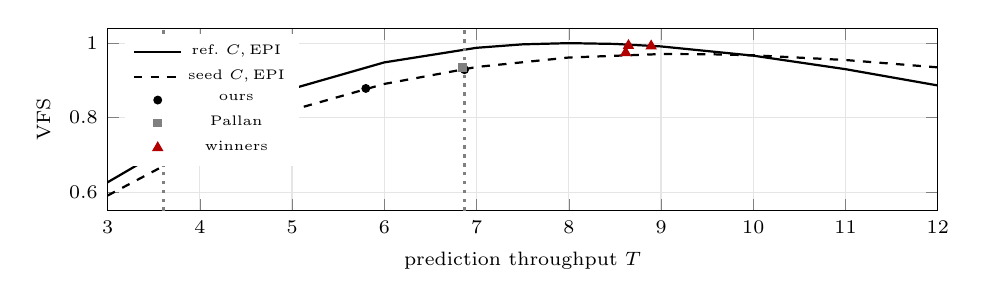
\begin{tikzpicture}
\begin{axis}[width=\columnwidth,height=3.9cm,
  xlabel={prediction throughput $T$}, ylabel={\vfs{}},
  xmin=3,xmax=12, ymin=0.55,ymax=1.04,
  legend columns=1,
  legend style={font=\tiny,at={(0.02,0.97)},anchor=north west,draw=none,fill=white},
  tick label style={font=\scriptsize}, label style={font=\scriptsize},
  grid=major, grid style={gray!20}]
\addplot[thick] coordinates
 {(3.0,0.6264) (4.0,0.7707) (5.0,0.8774) (6.0,0.9483) (7.0,0.9875) (7.5,0.9968)
  (8.0,1.0000) (8.5,0.9979) (9.0,0.9912) (10.0,0.9664) (11.0,0.9301)
  (12.0,0.8864)};
\addlegendentry{ref.\ $C,\epi{}$}
\addplot[thick,dashed] coordinates
 {(3.0,0.5908) (4.0,0.7216) (5.0,0.8204) (6.0,0.8905) (7.0,0.9360) (8.0,0.9614)
  (9.0,0.9707) (9.5,0.9704) (10.0,0.9674) (11.0,0.9547) (12.0,0.9350)};
\addlegendentry{seed $C,\epi{}$}
\addplot[only marks,mark=*,mark size=1.4pt] coordinates {(5.80,0.8784) (6.87,0.9288)};
\addlegendentry{ours}
\addplot[only marks,mark=square*,mark size=1.4pt,gray] coordinates {(6.844,0.9345)};
\addlegendentry{Pallan}
\addplot[only marks,mark=triangle*,mark size=2pt,red!70!black] coordinates
 {(8.617,0.9742) (8.647,0.9935) (8.893,0.9921)};
\addlegendentry{winners}
\addplot[gray,dotted,very thick,forget plot] coordinates {(3.61,0.55) (3.61,1.04)};
\addplot[gray,dotted,very thick,forget plot] coordinates {(6.87,0.55) (6.87,1.04)};
\end{axis}
\end{tikzpicture}
\caption{\vfs{} as a function of $T$ with $C$ and \epi{} held fixed (lines),
together with reported designs (marks). The dotted lines bracket every design
our search produced; the winning entries lie beyond the knee.}
\label{fig:tcurve}
\end{figure}

\subsection{Throughput dominance is a regime}

With the score in closed form, we can ask how sensitive it is to each input,
and Table~\ref{tab:elast} shows that the answer depends on where a design sits.
When $C$ and
\epi{} are held at their reference values, \vfs{} peaks at $T=8.05$. At that
peak the throughput elasticity is only $+0.008$ and accuracy ($-0.035$) is the
largest term; near the reference, the score is intentionally insensitive to
additional width.

The picture changes on the rising flank of Fig.~\ref{fig:tcurve}. Every design
our search produced lies in $T\in[3.61,6.87]$, with throughput elasticities
between $+0.28$ and $+0.68$, and in all 116 the throughput term exceeds the
accuracy term by a factor of $1.2$--$5.2$. Pallan's campaign occupied the same
region: the sensitivities he reports at $T=6.84$ ($+2.4\%$, $+1.4\%$, and
$+0.2\%$ \vfs{} for a 10\% change in $T$, mpi, and \epi{}) agree with
Eq.~\eqref{eq:vfs} evaluated at that point ($+2.2$, $+1.3$, $+0.2$).

The winning entries lie elsewhere. At their reported operating points the
throughput elasticity falls to between $-0.015$ and $+0.056$, while the accuracy
elasticity grows to between $-0.048$ and $-0.082$. MORSL and Fan in fact sit
almost exactly at the throughput that maximizes \vfs{} for their own $C$ and
\epi{} ($8.59$ and $8.78$), where further width would \emph{lower} the score.
They reached this region through ahead-pipelining~\cite{koizumi,fan,dang}, a
change that no resizing of the reference TAGE can express. The claim that
throughput dominates therefore describes the region that parameter search
explores, not \vfs{} itself, and an agent that internalizes it will keep buying
width well past the point at which width stops paying.

\subsection{What the flank selects}

The same effect is visible within our own population. Across the 116 designs,
\vfs{} correlates with $T$ at $r=+0.949$ but with \mpki{} at only $r=-0.113$,
even though \mpki{} varies from $5.08$ to $10.08$. The best design,
\texttt{gen037\_2}, differs from the seed chiefly by raising the block length
\texttt{LOGLB} from 6 to 7, so that each lookup covers 32 instructions rather
than 16, which is the same change Pallan's agents identified. Its \mpki{} barely
moves ($5.338\to5.333$) while $T$ rises from $5.80$ to $6.87$. Conversely, the
most accurate design we found (\mpki{} $5.084$) scores only $0.744$, and all
seven final elites sit at \texttt{LOGLB}$=7$, the upper bound of the template.

On this flank, accuracy behaves less like a slope that the search climbs than
like a cliff from which it occasionally falls. Widening the block consumes
hashed tag bits, leaving $H=\texttt{TAGW}-(\texttt{LOGLB}-2)$. The 100 designs
with $H\ge6$ average $5.43$ \mpki{} (at most $5.97$), whereas the 16 with $H\le5$
average $9.47$ (at least $9.00$).

\section{Can the Evaluators Be Trusted?}
\label{sec:res}

A score is only half of what an agent optimizes; the other half is the
machinery that measures it. Before trusting a loop's verdicts, we therefore put
two questions to its evaluators.

\subsection{Does each tier separate the population?}

The answer differs sharply between our two validation tiers. The port check
does its job. Although the rendered port departs structurally from Tier~0 (the
first prediction level is not ported, and ChampSim advances history per branch
rather than per block), all 40 promoted designs passed the gate with \mpki{}
1.5--8.8\% \emph{lower} than Tier~0 (ratios 0.912--0.985), a bias consistent
with the finer-grained history.

The gem5 tier, by contrast, cannot tell designs apart. Across the 39 designs it
evaluated, depth-9 core IPC ranged only from $0.8867$ to $0.8920$, a spread of
$0.60\%$ that stayed below $0.69\%$ at every depth and did not widen as the
population grew from 10 to 39 designs. Its correlation with \vfs{} is $r=+0.06$.
Its correlation with Tier-0 \mpki{}, $r=-0.73$, initially suggests agreement
between simulators, but it falls to $-0.27$ once a single outlier
(\texttt{gen005\_0}, \mpki{} $9.37$) is removed. Three short kernels are simply
too little workload to expose a 5\% difference in \mpki{}. The broader lesson is
that an expensive tier must first be shown to discriminate among the designs it
will actually see; ours had the appearance of validation without its substance.

\subsection{Does the ranking survive other depths?}

Pipeline depth enters \vfs{} only through Eq.~\eqref{eq:cpi}, so the score at
any depth can be recomputed in closed form from counters measured once. We
exploit this property to rank the seven archived elites at each depth and
compare the result with the ranking at $D=9$ using Kendall's $\tau$ over 21
pairs. Table~\ref{tab:tau} reports this comparison for the archives at
generations 10 and 39, which share no designs.

\begin{table}[t]
\caption{Kendall $\tau$ of the seven-elite ranking at depth $D$ against the
ranking at $D=9$, with the number of discordant pairs.}
\label{tab:tau}
\centering\footnotesize
\begin{tabular}{@{}rrrrr@{}}
\toprule
& \multicolumn{2}{c}{gen.\ 10 archive} & \multicolumn{2}{c}{gen.\ 39 archive} \\
\cmidrule(lr){2-3}\cmidrule(lr){4-5}
$D$ & $\tau$ & disc. & $\tau$ & disc. \\
\midrule
3        & $+1.000$ & 0 & $+0.905$ & 1 \\
6, 9, 12 & $+1.000$ & 0 & $+1.000$ & 0 \\
16       & $+0.905$ & 1 & $+1.000$ & 0 \\
20       & $+0.714$ & 3 & $+1.000$ & 0 \\
25, 30   & $+0.619$ & 4 & $+1.000$ & 0 \\
\bottomrule
\end{tabular}
\end{table}

The two archives behave very differently. At generation 10, every discordant
pair involves \texttt{gen006\_2}, the only elite with high \mpki{} ($9.22$,
against $5.08$--$5.46$ for the rest). Its tags had been cut to $H=4$ in exchange
for bandwidth, and it survived only because it held a cell of its own despite
scoring below the seed; removing it restores $\tau=+1$ at every depth. By
generation 39 this design had been evicted, the archive's \mpki{} range had
narrowed from $1.8\times$ to $1.09\times$, and the ranking is identical from
$D=6$ to $D=30$. Eq.~\eqref{eq:cpi} explains why: because $C$ scales with
$\text{mpi}\cdot D$, a design with $1.7\times$ the misprediction rate loses
ground $1.7\times$ faster as the pipeline deepens. Depth robustness is thus
governed by accuracy, precisely the term the flank discounts, and nothing in the
depth-9 score distinguishes the fragile archive from the robust one.

The held-out traces provide a final check. On them the generation-39 ranking is
preserved exactly ($\tau=+1.000$), even for its closest pair (0.0012 apart).
The result is weaker than it appears, however: every elite loses a nearly
constant $0.0287\pm0.0019$ on the harder traces, so only near-ties could have
swapped. The test rules out an ordering fitted to the search traces, not a
failure to transfer to unlike workloads.

\section{An LLM on the Search Space}
\label{sec:bounds}

These results point to a natural place for a language model. Every elite sits
at the \texttt{LOGLB} ceiling, a bound that was never justified, which suggests
that the shape of the search space may constrain the search as much as the
operator does. We therefore give an LLM control of the box rather than the
design. Before each generation, a bounds agent (Claude Opus~5) receives each
parameter's range, the current archive, the fraction of evaluated designs lying
on each bound, and its own earlier changes, and returns revised ranges together
with its reasons; a validator rejects ranges under which a hashed field could
underflow, though it never fired. The baseline is a rule that widens a bound by
one step whenever at least 25\% of evaluated designs lie on it. Both arms resume
from the generation-10 archive for generations 11--20 (30 proposals each) with
the same operator and random stream, so their proposals are paired and diverge
only where a bound clamps a mutation. The fixed-bounds run, offset by one
generation after a restart, is compared by outcome only; Tier~2 was off.

All three arms converge to the same optimum. By generation 20 they hold the same
best design ($\vfs{}=0.92878$, which the fixed-bounds run later improved by just
$0.00006$) and occupy seven cells each. Both adaptive arms raised the
\texttt{LOGLB} ceiling to 8, but the operator moved \texttt{LOGLB} in only 4 of
30 proposals and never upward from 7, so the experiment cannot tell whether that
ceiling was binding.

Where the arms differ is in how many evaluations they waste. Twenty of the 30
paired proposals are identical. Among the ten that differ, the LLM arm leads by
$+0.017$ to $+0.228$ in five, trails by at most $0.004$ in three, and ties in
two, for a mean paired gain of $+0.021$ (mean \vfs{} $0.796$ against $0.775$,
and $0.757$ with fixed bounds). The three largest gains all stem from the
agent's clamps (Table~\ref{tab:bounds}), and one of them avoids the tag-bit
cliff: the agent had derived $H$ from the template and cited it in its
reasoning. With a single seed and only ten differing pairs, however, these
results are descriptive rather than conclusive.

\begin{table}[t]
\caption{Paired proposals in which a bound clamp decided the outcome.}
\label{tab:bounds}
\centering\footnotesize
\begin{tabular}{@{}llrr@{}}
\toprule
Proposal & LLM clamp & rule \vfs{} & LLM \vfs{} \\
\midrule
gen014\_1 & \texttt{TAGW} $9\to10$ ($H$: $5\to6$) & $0.783$ & $0.872$ \\
gen016\_1 & \texttt{LOGP1} $16\to14$ & $0.667$ & $0.896$ \\
gen018\_0 & \texttt{LOGP1} $16\to14$ & $0.701$ & $0.929$ \\
\bottomrule
\end{tabular}
\end{table}

The agent's reasoning deserves as much scrutiny as its outcomes. Of its 12
changes, three widened a range and were never used, while nine narrowed ranges
toward the current elites, an exploitative habit at odds with the diversity the
archive exists to preserve; the rule made two changes and stopped. More revealingly, the agent
twice narrowed \texttt{GHIST} ($[40,400]\to[70,180]\to[90,130]$) on the grounds
that a tighter range lets ``proportional mutations'' reach further. The operator,
however, steps by $\pm1$ or $\pm2$ regardless of range, so the change could have
no effect, and indeed had none. The rationale was fluent and numerate, but it
described a loop the agent could not see. An agent that shapes a search space
should therefore be shown the operator that searches it, and the mechanism it
claims should be checked alongside its results.

\section{Discussion and Limitations}

Taken together, these results suggest a concrete test for future work. Pallan's
agents and our operator stalled on the same flank, whereas the winners escaped
it through an algorithmic change, so the key question for an LLM that proposes
designs is whether it can leave that flank. The throughput elasticity of its
designs (Table~\ref{tab:elast}) measures this directly: an agent still buying
width near $T\approx8.6$ is optimizing the lesson rather than the score.

Our study has several limitations. The operator cannot invent algorithms, and
our best score (0.9288) remains below Pallan's and every winner's; this paper is
an audit, not an entry. Other entries' operating points are self-reported under
their own settings, and MORSL's $C$ is inferred. Only $2\times2\times2$ of the
behavior grid's 144 cells are reachable, and Table~\ref{tab:tau} compares two
archives observationally rather than through an ablation.

\section{Conclusion}

\vfs{} is a genuine improvement over ranking predictors by misprediction rate,
but what it rewards depends on where a design stands: below the reference
throughput it rewards width, and near the reference it rewards accuracy. A loop
that experiences only the first regime will draw the wrong lesson from its own
success. We therefore recommend that agentic searches over cost-aware metrics
report the elasticities at the operating points they reach, demonstrate that
each evaluation tier separates their population, and report rankings at several
pipeline depths, which Eq.~\eqref{eq:cpi} makes essentially free. The loop is
open source at \url{https://github.com/zxc12523/chia}.

\section*{Acknowledgment}
% Required by the A^3 CFP.
Portions of this paper's text and analysis were drafted with AI assistance
(Claude Opus~5, Anthropic). The authors reviewed all content and take full
responsibility for it.

\balance
\begin{thebibliography}{99}
\bibitem{cbpng} A. Lindsay, P. Michaud, R. Sheikh, M. Madhav, and A. Alameldeen,
``The Next-Generation Championship in Branch Prediction (CBP-NG),'' held with
ISCA 2026. Simulator: \url{https://github.com/AmpereComputing/cbp-ng}.
\bibitem{harcom} P. Michaud, ``HARCOM: Hardware complexity model for
microarchitecture exploration,'' CBP-NG documentation, 2026.
\bibitem{vfsmetric} P. Michaud, ``A scoring metric for the CBP-NG
championship,'' CBP-NG documentation, 2026.
\bibitem{chia} A. Cui \emph{et al.}, ``CHIA: An open-source framework for
principled, agentic AI-driven hardware/software co-design research,''
arXiv:2606.27350, 2026.
\bibitem{pallan} M. Pallan, ``Coding agents as design searchers: An autonomous
TAGE tuning campaign for CBP-NG,'' in \emph{CBP-NG Workshop (ISCA)}, 2026.
\bibitem{koizumi} T. Koizumi \emph{et al.}, ``MORSL: Minimal-overhead
rank-based predictor with summation-free correction and lazy access,'' in
\emph{CBP-NG Workshop (ISCA)}, 2026.
\bibitem{fan} J. Fan, ``Enhance ahead-pipelined N-branch GShare with tagged
tables,'' in \emph{CBP-NG Workshop (ISCA)}, 2026.
\bibitem{dang} N. Dang and E. Rotenberg, ``An energy-efficient ahead-pipelined
TAGE branch predictor for CBP-NG,'' in \emph{CBP-NG Workshop (ISCA)}, 2026.
\bibitem{seznec2006tage} A. Seznec and P. Michaud, ``A case for (partially)
tagged geometric history length branch prediction,'' \emph{J. Instruction-Level
Parallelism}, vol. 8, 2006.
\bibitem{seznec2011tage} A. Seznec, ``A new case for the TAGE branch
predictor,'' in \emph{Proc. MICRO}, 2011.
\bibitem{jimenez2000delay} D. A. Jim\'enez, S. W. Keckler, and C. Lin, ``The
impact of delay on the design of branch predictors,'' in \emph{Proc. MICRO},
2000.
\bibitem{jimenez2003reconsidering} D. A. Jim\'enez, ``Reconsidering complex
branch predictors,'' in \emph{Proc. HPCA}, 2003.
\bibitem{champsim} N. Gober \emph{et al.}, ``The Championship Simulator:
Architectural simulation for education and competition,'' arXiv:2210.14324, 2022.
\bibitem{gem5} N. Binkert \emph{et al.}, ``The gem5 simulator,''
\emph{ACM SIGARCH Comput. Archit. News}, vol. 39, no. 2, 2011.
\bibitem{mouret2015illuminating} J.-B. Mouret and J. Clune, ``Illuminating
search spaces by mapping elites,'' arXiv:1504.04909, 2015.
\bibitem{alphaevolve} A. Novikov \emph{et al.}, ``AlphaEvolve: A coding agent
for scientific and algorithmic discovery,'' arXiv:2506.13131, 2025.
\bibitem{archgym} S. Krishnan \emph{et al.}, ``ArchGym: An open-source
gymnasium for machine learning assisted architecture design,'' in \emph{Proc.
ISCA}, 2023.
\bibitem{lehman2020surprising} J. Lehman \emph{et al.}, ``The surprising
creativity of digital evolution,'' \emph{Artificial Life}, vol. 26, no. 2, 2020.
\bibitem{amodei2016concrete} D. Amodei \emph{et al.}, ``Concrete problems in
AI safety,'' arXiv:1606.06565, 2016.
\end{thebibliography}

\end{document}
